% intro.tex:

\chapter{Introduction}

\section{AI and Edge Computing}
\label{chap:intro:ai_and_edge}

\ac{DNN}s currently represent the state of the art in complex regression and
classification problems in image recognition, sequence to sequence learning
\cite{dnn_is_sota_seq2seq}, speech recognition \cite{dnn_is_sota_speech}. As
such they are being deployed on both cloud platforms and edge devices at scale.

While DNN structures vary significantly \ac{CNN}s are a widely used variant of
\ac{DNN}s that demonstrate great accuracy in image/video recognition. The main
computation layer of \ac{CNN}s that consumes most of the runtime of a network is
the convolutional layer. A convolution layer operates on multi-dimension tensors
as part of a \ac{CNN}s feature extraction portion of the network. Convolution
layers exhibit a significant amount of parallel behavior and data reuse.
Additionally, the tight latency, throughout and energy constraints imposed on
CNN's in various environments, particularly on edge devices has led to the
proliferation of customized hardware accelerators for \ac{CNN}s with particular
emphasis on accelerating convolution layers. 


\section{Convolution accelerators}
\label{chap:intro:cnn_accelerator_design_approaches}

Prior work on \ac{CNN} accelerators design can broadly be
classified based on 1) what they are implemented as: hardened \ac{ASIC}s/ or
synthesized accelerated in \ac{FPGA} fabrics 2)
what they accelerate, either entire layers of the network or
specifically convolution layers and finally 3) Their mathematical interpretation
of the convolution operation as either fundamentally a matrix operation post
reorganization of its input tensor or as a conventional stencil based operation.

Regardless of the target execution platform chosen for a novel \ac{CNN}
accelerator architecture there exists a need to create a general enough
architecture that can support a wide variety of networks and network layer
types. \ac{CNN} \ac{ACC} generality can be decomposed into 1) Convolution
generality, which can be defined as the range of support convolution layers and
2) Network generality, which can be defined as the types convolution network
layers supported 

\ac{FPGA}s inherently have an advantage with respect to both types of generality given
their reconfigurable nature. \ac{FPGA}-centric approaches incorporate the
architecture of a target \ac{CNN} network into their architecture compilation
process \cite{caffeine}. This allows \ac{FPGA}-based architectures to tackle
network generality by adding layer-specific accelerators (provided they are
available) at compile time, as well as tailor \ac{Conv} \ac{ACC} primitives to
the target network in order to provide the appropriate amount of \ac{Conv}
generality and performance. The disadvantage of \ac{FPGA} based architectures is
1) The need to recompile the architecture prior to deployment of a new \ac{CNN}
with possibly no support for a new \ac{CNN} without recompilation 2) Inferior performance and energy
efficiency compared to a hardened architecture. One could harden a design
produced by an \ac{FPGA}-based architecture compilation process. However, this
will produce a design optimized for only one network and may not be general
enough. To the best of this author's knowledge, no \ac{FPGA}-based \ac{ACC}
compilation processes incorporate more than one \ac{CNN} network architectures
into their architecture optimization process. 

\ac{ASIC}-based architectures tackle network generality by introducing a wide
variety of hardened layer accelerator primitives on-chip \cite{tpu}.
Additionally, they tackle convolution generality by either 1) Reinterpreting
convolution layers as \ac{GEMM} operations or 2) Creating a general
enough \ac{Conv} \ac{ACC} capable of supporting a wide range of \ac{Conv} layer
dimensions directly \cite{eyerissv2}. Given the pace of development in \ac{DNN}s,
new layers like \cite{transformer_model}'s self attention layer can
arise and become integral to improving \ac{DNN} model performance
\cite{conv_and_transformers}. These new layers may not be fully compatible with
the chosen accelerator primitives in the \ac{ASIC}-based design approach and as
a result may only be partially accelerated. Additionally, \ac{ASIC}-based
designs must balance their dedication of on-chip resources to convolution vs
other resource intensive layers (e.g \ac{FC} layers) which may cause convolution
performance to suffer. Approaches that reinterpret convolutions to increase
convolution generality like \ac{GEMM} tend to dramatically increase data volume
which may strain on-chip memory resources as well as decrease energy efficiency
\cite{caffeine}. Finally, supporting a wide range of convolutions can come at
the cost of reduced performance/ energy efficiency for the statistical common
case of convolutions layer dimensions in a wide range of \ac{CNN}s.  

\section{Problem Definition}
\label{chap:intro:prob_def}

The literature demonstrates a need to create an ASIC-based convolution
accelerator, one that offers improved performance and energy efficiency for the
common case of convolution layers across a broad range of \ac{CNN}s. This
ASIC-based convolution accelerator would also need to maintain operational generality
to support a wide variety of layer types found in many modern DNNs without sacrificing
performance. 

To optimize for the common case of convolutions this accelerator we need to find the
common case of convolution layers in a broad range of networks. This will allow
us to determine how to optimize the accelerator's memory hierarchy and on-chip
network structure.   

Additionally, given the wide variety of DNNs available, the
architecture would need to be sufficiently configurable at compile time to allow
optimization of it's structure based on changing trends in network
architectures in the literature. 

On-chip data movement should be flexible enough to allow the mapping of
diverse layers to the architecture, but a purely static communication and memory
hierarchy structure won't be enough to satisfy that requirement. Therefore, the
architecture would need to use programmable on-chip data movement primitives. To
program these primitives, a network compiler would need to be developed. The
compiler would be used to generate data movement instructions for the on-chip
data movement primitives based on layer configuration within the network.   

Finally, in order to estimate the performance and energy metrics of this accelerator, a
cycle accurate simulator would need to be developed to allow the assessment of
different configurations of the architecture on a wide variety of networks. 

\section{Solution Overview}
\label{chap:intro:solution_overview}

\begin{figure}[!ht]
  \centering
  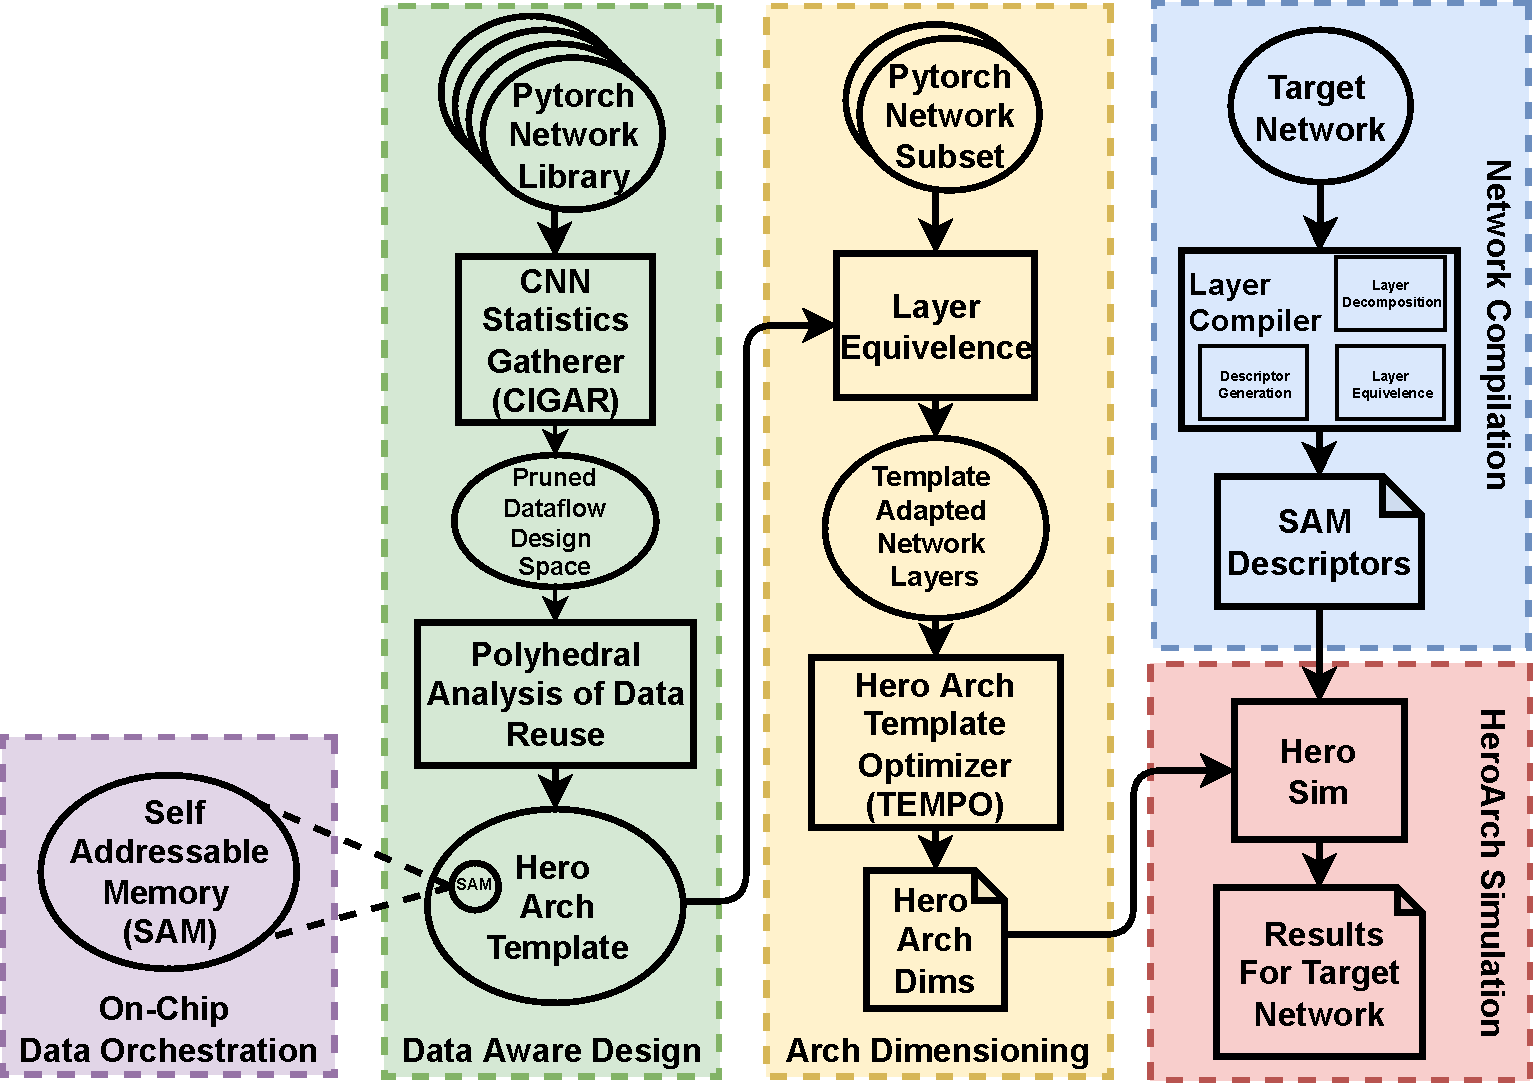
\includegraphics[scale=1]{fig/intro.pdf}
  \caption{Visual illustration of the solution overview}
  \label{fig:intro}
\end{figure}

This thesis presents (HERO), a Hybrid GEMM and Direct Convolution Accelerator.  
HERO supports general matrix multiplication to maintain generality across
different network layers. General matrix multiplication is the backbone of many
computationally intensive layers in modern DNNs, for example, self attention
layers in transformer networks \cite{transformer_model} as well as fully
connected layers in many CNNs like Resnet \cite{resnet}. Extending support to
GEMM should not detract from the primary goal of accelerating convolutions since
they represent a larger portion of most network's runtime.  
HERO is derived from a data aware design process. HERO is optimized for the
common case of convolutions in the literature by supporting these convolution
configurations directly without the need to convert them into GEMM using data
transformation techniques like Im2Col. To find the common case of convolutions,
this thesis introduces \ac{CIGAR}. CIGAR can gather configuration statistics for
convolution and linear layers in a libray of DNNs networks written in PyTorch
\cite{pytorch}. The heart of CIGAR is it's model dim collector that can collect
convolution and linear layer configuration for any network written in pytorch.
CIGAR can analyze a network or a library of networks and reveal the most common
convolution layer configurations (e.g their kernel and stride sizes) across the
entire library. The networks analyzed by CIGAR are all provided by the \ac{TIMM}
python library of networks \cite{timm}, which has over 695 networks written in
pytorch available for analysis. Convolution layer configurations that are not
supported directly by the architecture are converted into equivalent GEMM
operations using data transformation techniques like Im2Col
\cite{cafe_con_troll}. 

HERO's memory hierarchy and on chip communication is optimized for on-chip data
reuse. To determine reuse behavior this thesis applies the polyhedral model to
analyze the reuse behavior of different data elements in the convolution
algorithm using the technique in \cite{meeus}.

HERO is more than a single architecture. HERO represents a configurable template
with flexible allocation of on chip compute resources for processing convolution
layer channels and filters. This configurability allows for compile time
optimization of HERO by changing the number of PEs allocated to processing
different channels and filters in a convolution layer. To determine the optimal
configuration this thesis introduces \ac{TEMPO}. TEMPO uses analytical models
for estimating different architecture metrics like latency, utilization and
memory access counts when running different DNNs. To be able to estimate these
metrics TEMPO takes advantage of CIGAR's model dimension collection to extract
configurations of convolution layers and applies the aforementioned analytical
models to them.   
TEMPO provides the initial architecture dimensions for the HERO Template in
order to get the first estimates for other performance metrics. TEMPO only
defines layer dims for channel and filter concurrency. A separate analysis of
memory usage for different convolution elements is provided in this thesis. Data
for the memory usage is provided by CIGAR.   
The networks subset used by TEMPO is the entire TIMM library find the most
general arch dims for HERO. 

To manage data movement inside HERO this thesis introduces \ac{SAM}s which are
on-chip programmable memory primitive used for data orchestration. SAMs are
programmed using descriptor that defined time dependent address streams.
Combining SAMs with sufficiently flexible on-chip communication provides the
necessary flexibility to map arbitrary network layers onto HERO. 

To map different networks to a HERO instance, this thesis introduces
\ac{EMPIRE}. EMPIRE takes the configuration layers of pytorch networks and
compiles them down to data movement descriptors for the SAMs in HERO.
\ac{EMPIRE} is composed of two compilation phases. The first phase tansforms
layers unsupported by HERO in a network to supported layers. The second phase
generates data movement descriptors for HERO's on-chip SAMs from the supported
layer's configuration.
   
To evaluate the power and performance of different HERO configurations this
thesis introduces HERO-sim. HERO-sim is a cycle simulation framework for HERO
with a SystemC backend for cycle accurate simulation of HERO coupled with a
python backend for interfacing with models written in pytorch. HERO-sim can
generate power and performance metrics for different configurations of HERO when
running arbitrary PyTorch networks. 

The full solution overview is presented in \autoref{fig:intro}.

\section{Thesis Structure}
\label{chap:intro:thesis_structure}

\autoref{chap:background:intro} discusses background and related work in the
literature. \autoref{chap:dda} introduces \ac{CIGAR} and the data aware design
approach from which \ac{HERO} is derived. \autoref{chap:arch_dimensioning}
introduces \ac{TEMPO} from which several candidate configurations of HERO are
presented. \autoref{chap:data_orchestration} introduces the SAM primitive.
\autoref{chap:net_compile} discusses HERO's network compilation process and how
SAM descriptor are generated from arbitrary models in Pytorch using \ac{EMPIRE}.
Finally \autoref{chap:hero:sim_platform} discusses the HERO simulation platform
as well as results from running a HERO configuration optimized by TEMPO on all
695 networks in the TIMM library. 

